\section{Mirror-Twin Inversion Locks Gems into Vertical Towers}
\label{sec:stacking}

Our final mechanical investigation treats Magic Gems as physical building blocks under gravity. When a polyhedron $\mathcal G_\lambda(S)$ rests on a flat horizontal table on one of its facets $F$, or when multiple gems are stacked face-to-face into a vertical column, two geometric questions arise: (i)~when is a resting facet statically stable against tipping under gravity, and (ii)~how can copies of a gem be stacked along slanted facets without the column curving away from the vertical and toppling?

\subsection{Cubic Aspect Scaling Raises Facet Resting Stability from \texorpdfstring{$43.0\%$}{43.0\%} to \texorpdfstring{$74.5\%$}{74.5\%}}

Let $F\subset\partial\mathcal G_\lambda(S)$ be a facet with outward unit normal $\hat{\mathbf n}_F(\lambda)$. When $\mathcal G_\lambda(S)$ rests with $F$ on a horizontal plane (so $\hat{\mathbf n}_F(\lambda)$ points straight down), gravity acts vertically through the centre of mass $\mathbf c(\lambda)$. Let $\pi_F(\mathbf c(\lambda))$ denote the orthogonal projection of $\mathbf c(\lambda)$ onto the affine plane of $F$, and let $h_F(\lambda)=(\mathbf p_F-\mathbf c(\lambda))\cdot(-\hat{\mathbf n}_F(\lambda))>0$ be the height of the centre of mass above the table.

\begin{definition}[Static stability margin and critical tipping angle]
\label{def:stability}
For a facet $F\subset\partial\mathcal G_\lambda(S)$, the \emph{stability margin} $d_{\mathrm{stab}}(S,F;\lambda)$ is the signed Euclidean distance in the plane of $F$ from $\pi_F(\mathbf c(\lambda))$ to the boundary $\partial F$ of the facet polygon (taken positive when $\pi_F(\mathbf c(\lambda))$ lies in the strict relative interior of $F$, and negative outside). Facet $F$ is \emph{statically stable} if and only if $d_{\mathrm{stab}}(S,F;\lambda)>0$, in which case its \emph{critical tipping angle} (the maximum tilt of the table before $\mathcal G_\lambda(S)$ topples across an edge of $F$) is
\begin{equation}
\label{eq:tip-angle}
\theta_{\mathrm{tip}}(S,F;\lambda) = \arctan\!\left(\frac{d_{\mathrm{stab}}(S,F;\lambda)}{h_F(\lambda)}\right).
\end{equation}
\end{definition}

\begin{proposition}[Order-four resting stability census]
\label{prop:stability-census}
Across all $880$ magic squares of order~$4$, the gems $\mathcal G_\lambda(S)$ possess a total of $14{,}824$ facets (mean $16.85$ facets per gem).
\begin{enumerate}
\item At the canonical lift $\lambda=1$, using the exact uniform-solid centre of mass $\mathbf c_0(S)$, exactly $6{,}378$ of the $14{,}824$ facets ($43.0\%$) are statically stable, with every gem possessing between $4$ and $12$ stable resting facets (mean $7.25$; using the balanced point centroid $O$ gives $6{,}340$ stable facets, $42.8\%$).
\item At the cubic 3D-print scale $\lambda_{\mathrm{cube}}=1/5=0.20$ (where the height span of $1,\dots,16$ equals the $3\times3$ grid footprint), the reduced vertical aspect ratio brings the centre of mass closer to the slanted upper and lower facets: $11{,}044$ of the $14{,}824$ facets ($74.5\%$) are statically stable, with a mean critical tipping angle of $17.8^\circ$ and a maximum of $47.3^\circ$ (\Cref{fig:mirror-stacking}(d)).
\end{enumerate}
\end{proposition}

\begin{proof}
For each of the $880$ gems and each facet $F\subset\partial\mathcal G_\lambda(S)$ with exact integer plane equation $aX+bY+cZ+d=0$ in doubled coordinates, rescaling $z\mapsto\lambda z$ transforms the outward normal to $\mathbf n_F(\lambda)\propto(a\lambda,b\lambda,c)$ and the solid centroid to $\mathbf c_0(\lambda)=(c_{0,x},c_{0,y},\lambda c_{0,z})$. Projecting $\mathbf c_0(\lambda)$ onto an orthonormal basis of the affine plane of $F$ and evaluating the signed edge distances $d_{\mathrm{stab}}(S,F;\lambda)$ and \eqref{eq:tip-angle} across all $14{,}824$ facets at $\lambda=1$ and $\lambda=0.20$ yields the stated counts and extremal angles.
\end{proof}

\subsection{Central Inversion Pairs Every Upper Facet with a Parallel Lower Facet of Its Mirror Twin}

Suppose we wish to stack multiple blocks vertically along an upper facet $F_+\subset\mathcal G_\lambda(S)$ (with outward normal $\mathbf n_+$, $n_{+,z}>0$) and a lower facet $F_-\subset\mathcal G_\lambda(S)$ (with outward normal $\mathbf n_-$, $n_{-,z}<0$). Stacking translated copies of the \emph{same} gem $\mathcal G_\lambda(S)$ without rotation requires $\mathbf n_-=-\mathbf n_+$ (which holds for only $124$ of the $880$ gems); when $\mathbf n_-\ne-\mathbf n_+$, same-gem copies meet at an open wedge gap (\Cref{fig:mirror-stacking}(c), left). Pairing a gem with its \emph{rotational complement (mirror twin)}
\begin{equation}
\label{eq:mirror-twin}
S^* := r^2\overline S = (N+1)\mathbf 1 - r^2 S
\end{equation}
solves the stacking problem universally via central inversion in $\R^3$ (\Cref{fig:mirror-stacking}(a,c)).

\begin{figure}[htbp]
\centering
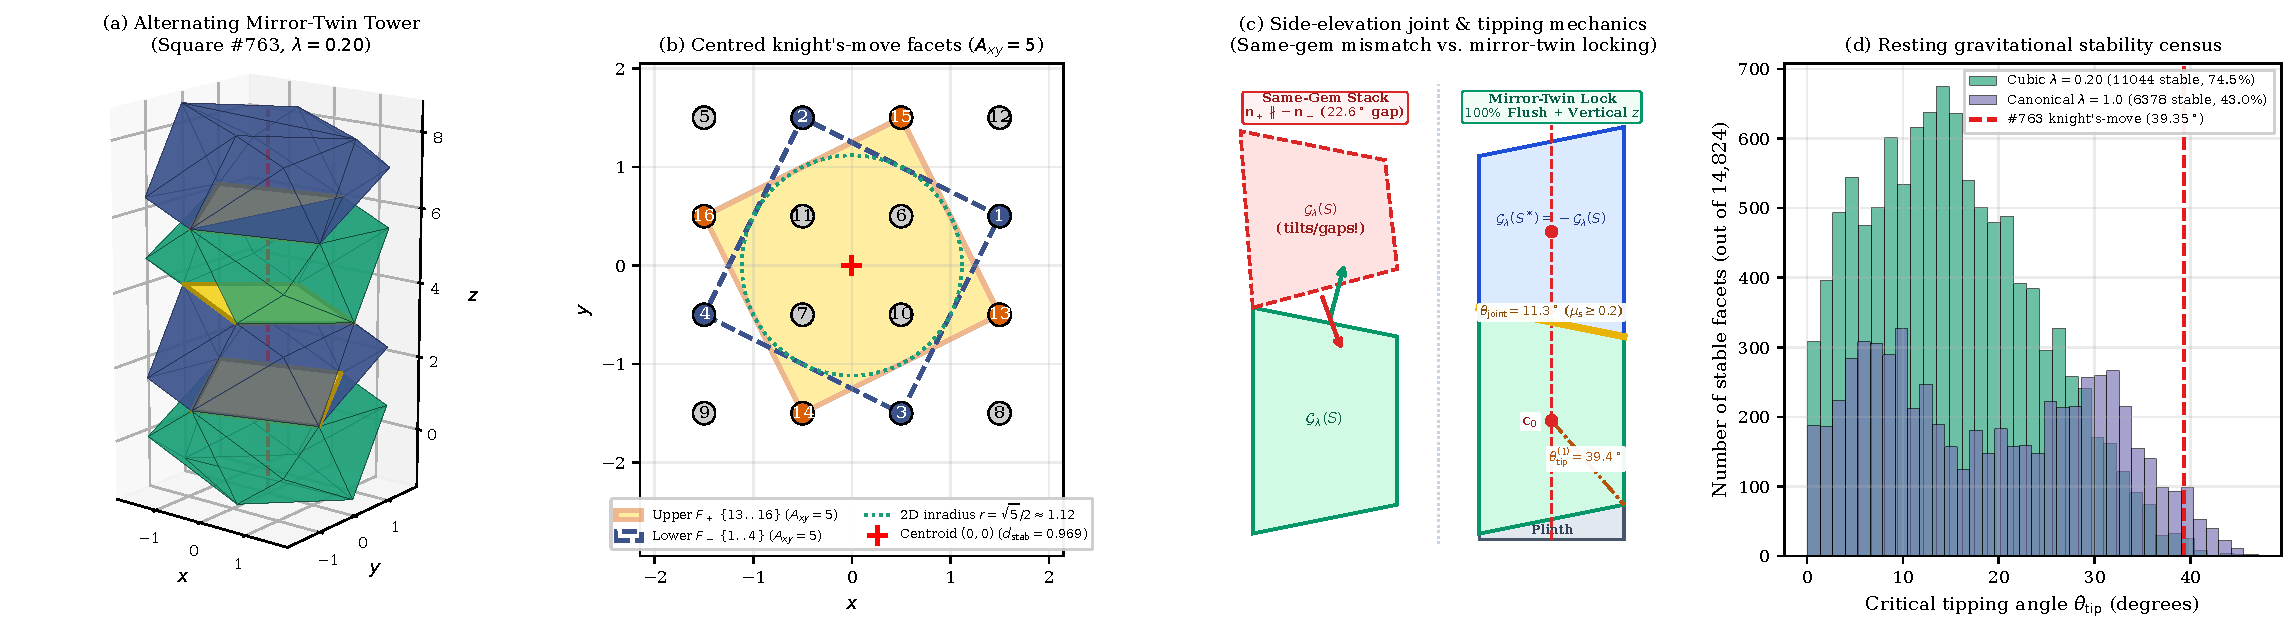
\includegraphics[width=\textwidth]{figures/fig_mirror_stacking.pdf}
\caption{Mirror-twin facet locking and periodic vertical towers. (a)~Four-block alternating tower of square \#763 at the cubic 3D-print scale $\lambda=0.20$, alternating $\mathcal G_\lambda(S)$ (green) with its mirror twin $\mathcal G_\lambda(r^2\overline S)=-\mathcal G_\lambda(S)$ (blue); the golden contact joints are the centred knight's-move squares $\{13,14,15,16\}$ and $\{1,2,3,4\}$, which meet with $100\%$ vertex congruence and keep the column's centre of mass on the vertical $z$-axis (red dashed). (b)~Top-down $(x,y)$ footprint of square \#763 showing the dual knight's-move squares of area $A_{xy}=5$ and 2D footprint inradius $r=\sqrt{5}/2\approx1.12$ (while the 3D tilted-plane stability margin from $\mathbf c_0$ is $d_{\mathrm{stab}}=0.969$ at $\lambda=0.20$). (c)~Two-dimensional side-elevation joint and tipping schematic comparing the $2\theta_{\mathrm{joint}}=22.6^\circ$ wedge mismatch of unrotated same-gem stacking against flush mirror-twin locking ($\mathbf n_+^*=-\mathbf n_+$) on a $\theta_{\mathrm{joint}}=11.3^\circ$ base plinth. (d)~Census of critical tipping angles $\theta_{\mathrm{tip}}$ over all $14{,}824$ facets at $\lambda=0.20$ and $\lambda=1.0$.}
\label{fig:mirror-stacking}
\end{figure}

\begin{theorem}[Mirror-Twin Inversion and Zero-Rotation Alternating Towers]
\label{thm:mirror-tower}
Let $S$ be any arrangement of order $n$, let $S^*=r^2\overline S$ be its half-turned complement, and let $\lambda>0$.
\begin{enumerate}
\item \emph{(Central inversion identity.)} In $\R^3$, the lifted point clouds and convex hulls satisfy
\begin{equation}
\label{eq:central-inv}
P_{S^*}(\lambda) = -P_S(\lambda),\qquad
\mathcal G_\lambda(S^*) = -\mathcal G_\lambda(S).
\end{equation}
Consequently, the map $F\mapsto F^*:=-F$ is an area-preserving, normal-reversing bijection between the upper facets $F_+\subset\mathcal G_\lambda(S)$ (outward normal $+\mathbf n_+$) and the lower facets $F_+^*\subset\mathcal G_\lambda(S^*)$ (outward normal $-\mathbf n_+$), and between the lower facets $F_-\subset\mathcal G_\lambda(S)$ (outward normal $+\mathbf n_-$) and the upper facets $F_-^*=-F_-\subset\mathcal G_\lambda(S^*)$ (outward normal $-\mathbf n_-$).
\item \emph{(Zero-rotation alternating tower.)} Choose \emph{any} upper facet $F_+\subset\mathcal G_\lambda(S)$ and \emph{any} lower facet $F_-\subset\mathcal G_\lambda(S)$ (not necessarily parallel) that are centrally symmetric polygons in $\R^3$ with centroids $\mathbf c(F_+)$ and $\mathbf c(F_-)$. Define the alternating sequence of unrotated blocks $B_0,B_1,B_2,\dots$ by
\begin{equation}
\label{eq:tower-blocks}
B_{2m} = \mathcal G_\lambda(S) + m\mathbf T,\qquad
B_{2m+1} = -\mathcal G_\lambda(S) + 2\mathbf c(F_+) + m\mathbf T,\qquad
\mathbf T = 2\bigl(\mathbf c(F_+) - \mathbf c(F_-)\bigr).
\end{equation}
Then:
\begin{enumerate}
\item At every odd joint $B_{2m}\cap B_{2m+1}$, the upper facet $F_+ + m\mathbf T$ of $B_{2m}$ coincides \emph{identically} (100\% polygon and vertex overlap, with opposite outward normals $\pm\mathbf n_+$) with the lower facet $-F_+ + 2\mathbf c(F_+) + m\mathbf T$ of $B_{2m+1}$.
\item At every even joint $B_{2m-1}\cap B_{2m}$, the upper facet $-F_- + 2\mathbf c(F_+) + (m-1)\mathbf T$ of $B_{2m-1}$ coincides \emph{identically} (with opposite outward normals $\mp\mathbf n_-$) with the lower facet $F_- + m\mathbf T$ of $B_{2m}$.
\item Every two-block repeating unit $B_{2m}\cup B_{2m+1}$ is centrally symmetric about $\mathbf c(F_+)+m\mathbf T$. When $\mathbf c(F_+)=(0,0,z_+)$ and $\mathbf c(F_-)=(0,0,z_-)$ both lie on the vertical $z$-axis ($z_+>0>z_-$), the period vector $\mathbf T=(0,0,2(z_+-z_-))$ is purely vertical, and the centre of mass of any $2M$-block tower lies on the $z$-axis regardless of whether $\mathbf c_0(S)=\mathbf 0$ (\Cref{fig:mirror-stacking}(a,c)).
\end{enumerate}
\end{enumerate}
\end{theorem}

\begin{proof}
(1) In centred coordinates \eqref{eq:coords}, $r^2$ sends $(x,y)\mapsto(-x,-y)$ and complementation sends $z\mapsto-z$, so $r^2\overline S$ lifts to $-\mathbf p_{ij}(\lambda)$, proving \eqref{eq:central-inv}.

(2) Central symmetry of $F_\pm$ about $\mathbf c(F_\pm)$ gives $-F_\pm + 2\mathbf c(F_\pm)=F_\pm$. Translating by $m\mathbf T$ yields~(2a) and~(2b), while central inversion about $\mathbf c(F_+)+m\mathbf T$ exchanges $B_{2m}$ and $B_{2m+1}$, proving~(2c).
\end{proof}

\subsection{Seventeen Gems Form Area-\texorpdfstring{$5$}{5} Towers via Centred Knight's-Move Square Facets}

\begin{proposition}[Vertically centered tower census and the knight's-move square \#763]
\label{prop:knights-move}
Across the $880$ magic squares of order~$4$:
\begin{enumerate}
\item Exactly $48$ squares possess both an upper facet $F_+$ and a lower facet $F_-$ that are centrally symmetric polygons whose centroids lie on the vertical axis $(0,0,z_\pm)$.
\item The maximum projected horizontal contact area among these $48$ squares is $A_{xy}=5$ (spanning $5/9\approx55.6\%$ of the $3\times3$ grid footprint), achieved by exactly $17$ squares (listed in \Cref{tab:knights-move}; e.g.\ squares \#603, \#763, and \#774). In all $17$ squares, the projected polygon $\pi_{xy}(F_+)$ is the centred $2\times1$ knight's-move square with vertices $(\pm\frac32,\mp\frac12)$ and $(\pm\frac12,\pm\tfrac32)$ (\Cref{fig:mirror-stacking}(b)).
\item Of these $17$ knight's-move gems, only two (\#774 and \#792) have parallel top and bottom facets ($\mathbf n_-=-\mathbf n_+$). The remaining $15$ gems cannot form a vertical column from unrotated copies of a single gem, but lock into a purely vertical, zero-drift column when alternated with their mirror twin.
\item In particular, square \#763 (Dudeney Group~VI, $\overline S=hS$, so $S^*=r^2\overline S=vS$ is its vertical reflection) is obtained from naturally balanced solid \#756 ($\mathbf c_0=\mathbf 0$, \Cref{tab:three-exceptions}) by swapping the single complementary pair $(4,13)\leftrightarrow(16,1)$ in rows~$2$--$3$ (\Cref{fig:hero-squares}(f)):
\[
S_{\#763} = \begin{pmatrix}
5 & 2 & \mathbf{15} & 12\\
\mathbf{16} & 11 & 6 & 1\\
4 & 7 & 10 & \mathbf{13}\\
9 & \mathbf{14} & 3 & 8
\end{pmatrix},\qquad
S^*_{\#763} = vS_{\#763} = \begin{pmatrix}
9 & 14 & 3 & 8\\
4 & 7 & 10 & 13\\
16 & 11 & 6 & 1\\
5 & 2 & 15 & 12
\end{pmatrix}.
\]
This single swap lifts $\{13,14,15,16\}$ onto the Pythagorean upper knight's-move plane $4x-3y+5z=30$ (centroid $(0,0,6\lambda)$) and $\{1,2,3,4\}$ onto the lower plane $-4x-3y-5z=30$ (centroid $(0,0,-6\lambda)$), while shifting the solid centroid slightly to $\mathbf c_0=(0,-5/126,0)$ (which cancels pairwise in $B_{2m}\cup B_{2m+1}$). Both facets have 3D area $5\sqrt{1+\lambda^2}$ ($\sqrt{26}\approx5.099$ at $\lambda=0.20$), stability margin $d_{\mathrm{stab}}=0.9694$, and single-block tipping angle $\theta_{\mathrm{tip}}^{(1)}=39.35^\circ$ at $\lambda=0.20$. Because $\mathbf n_\pm(\lambda)\propto(\pm4\lambda,-3\lambda,\pm5)$ makes angle $\theta_{\mathrm{joint}}(\lambda)=\arctan(\lambda)$ with $\hat{\mathbf e}_z$ ($\sqrt{4^2+(-3)^2}=5$), scaling from $\lambda=1$ ($\theta_{\mathrm{joint}}=45^\circ$) to $\lambda=0.20$ reduces the joint slope to $\arctan(0.20)\approx11.31^\circ$: any material with static friction $\mu_s>\lambda=0.20$ holds the unbonded column at level ($\theta_{\mathrm{table}}=0$), while tilting an $M$-block column of centre-of-mass height $H_M$ is governed by $\min\bigl(\arctan(\mu_s)-\theta_{\mathrm{joint}}(\lambda),\,\arctan(d_{\mathrm{stab}}/H_M)\bigr)$ (\Cref{fig:mirror-stacking}(c)).
\end{enumerate}
\end{proposition}

\begin{proof}
Testing each facet $F\subset\partial\mathcal G_1(S)$ across the $880$ gems for central symmetry ($F=2\mathbf c(F)-F$ with $c_x(F)=c_y(F)=0$) identifies the $48$ gems in~(1) and the $17$ gems of projected shoelace area $A_{xy}=5$ in~(2)--(3). For square \#763, substituting the lifted coordinates of $\{13,14,15,16\}$ and $\{1,2,3,4\}$ into $4x-3y+5(z/\lambda)=30$ and $-4x-3y-5(z/\lambda)=30$ verifies the facet planes, normals $\mathbf n_\pm(\lambda)\propto(\pm4\lambda,-3\lambda,\pm5)$, surface area $A_{xy}\sqrt{1+(4^2+3^2)\lambda^2/5^2}=5\sqrt{1+\lambda^2}$, and joint tilt $\tan\theta_{\mathrm{joint}}(\lambda)=\sqrt{(4\lambda)^2+(-3\lambda)^2}/5=\lambda$.
\end{proof}

\begin{remark}[Three-dimensional chirality and why a single mold cannot build the \#763 tower]
\label{rem:chirality}
Because square \#763 satisfies $\overline S=hS$ ($z(-x,y)=-z(x,y)$), its 3D gem $\mathcal G_\lambda(S_{\#763})$ is invariant under the $180^\circ$ proper rotation around the $y$-axis, $R_{y,\pi}(x,y,z)=(-x,y,-z)\in SO(3)$, which exchanges $F_+\colon 4x-3y+5z=30$ and $F_-\colon -4x-3y-5z=30$ and returns the \emph{exact same block} in its original orientation. Why, then, can a maker not cast two identical copies of $\mathcal G_\lambda(S_{\#763})$ from a single mold and flip the second block upside-down around the $x$-axis via $R_{x,\pi}(x,y,z)=(x,-y,-z)$ to mate with $F_+$? Because $R_{x,\pi}$ maps $F_+$ to a lower facet with outward normal $(+4\lambda,+3\lambda,-5)\ne-\mathbf n_+=(-4\lambda,+3\lambda,-5)$ (reversing the $y$-slope while keeping the $x$-slope at $+4\lambda$) and maps $F_-$ to an upper facet with outward normal $(-4\lambda,+3\lambda,+5)$. More fundamentally, the full orthogonal symmetry group of $\mathcal G_\lambda(S_{\#763})$ is $\operatorname{Aut}_{O(3)}\bigl(\mathcal G_\lambda(S_{\#763})\bigr)=\{I_3,R_{y,\pi}\}\cong C_2\subset SO(3)$, which contains no improper reflections: $\mathcal G_\lambda(S_{\#763})$ and its mirror twin $\mathcal G_\lambda(S^*_{\#763})=-\mathcal G_\lambda(S_{\#763})$ are \emph{chiral 3D enantiomorphs} lying in disjoint proper rigid-motion orbits ($R\mathcal G_\lambda(S_{\#763})\ne\mathcal G_\lambda(S^*_{\#763})$ for all $R\in SO(3)$). Building the alternating tower of \Cref{fig:mirror-stacking}(a) therefore genuinely requires two opposite-handed molds.
\end{remark}

\begin{table}[htbp]
\centering
\caption{Representative order-four Magic Gems from the $17$ classes (\#603, \#763, \#768, \#774, \#779, \#785, \#788, \#791, \#792, \#818, \#824, \#828, \#836, \#837, \#839, \#842, \#844) achieving the maximum projected contact area $A_{xy}=5$ via centred knight's-move square facets $F_+$ and $F_-$ (\Cref{prop:knights-move}). Plane equations $(a,b,c,d)$ are given in doubled coordinates $aX+bY+cZ+d=0$. ``Same-gem $\parallel$'' indicates whether $\mathbf n_-=-\mathbf n_+$; stability margins $d_{\mathrm{stab}}$ and single-block critical tipping angles $\theta_{\mathrm{tip}}^{(1)}$ (\Cref{def:stability}) are reported for the upper facet at $\lambda=0.20$.}
\label{tab:knights-move}
\small
\setlength{\tabcolsep}{4.5pt}
\begin{tabular}{r r c c c c c c}
\toprule
1-idx & 0-idx & Group & Upper $F_+$ plane & Lower $F_-$ plane & Same-gem $\parallel$ & $d_{\mathrm{stab}}$ ($\lambda=0.2$) & $\theta_{\mathrm{tip}}^{(1)}$ ($\lambda=0.2$)\\
\midrule
\#603 & 602 & VI & $(2,-9,5,-50)$ & $(-2,-9,-5,-50)$ & No  & $1.020$ & $45.39^\circ$\\
\#763 & 762 & VI & $(4,-3,5,-60)$ & $(-4,-3,-5,-60)$ & No  & $0.969$ & $39.35^\circ$\\
\#768 & 767 & II & $(0,-1,1,-12)$ & $(-4,-3,-5,-60)$ & No  & $0.973$ & $39.24^\circ$\\
\#774 & 773 & VI & $(1,0,1,-12)$  & $(-1,0,-1,-12)$  & Yes & $0.931$ & $38.35^\circ$\\
\#791 & 790 & VI & $(-3,-4,5,-60)$& $(-3,4,-5,-60)$  & No  & $0.969$ & $39.35^\circ$\\
\#792 & 791 & VI & $(0,-1,1,-12)$ & $(0,1,-1,-12)$   & Yes & $0.931$ & $38.35^\circ$\\
\#837 & 836 & VI & $(4,-3,5,-60)$ & $(4,3,-5,-60)$   & No  & $0.962$ & $38.94^\circ$\\
\bottomrule
\end{tabular}
\end{table}
